\section{Risultati Sperimentali}
Verranno elencati in questa sezione i risultati sperimentali, essi
sono estremamente dipendenti da un numero enorme di fattori di configurazione
e utilizzo, prima fra tutti la scelta del metodo di improvvisazione da parte
del musicista.

\subsection{Algoritmo a scelta casuale}
L'algoritmo a scelta casuale, come indicato nella sezione \ref{sec:musician_think},
soffre estremamente la mancanza di un database di pattern ben costruito
\footnote{purtroppo sia per mancanza di conoscenza strumentale
(per esempio riguardo all'organo), sia per mancanza temporale,
il database è decisamente scarno per utilizzi più avanzati di un semplice
\textbf{proof of concepts}};
\\
\todo{qua ci va la figura dell'organo}
questo si può notare immediatamente con un riscontro uditivo,
gli strumenti che possiedono un database di pattern ristretto tenderanno
a fare scelte sempre più casuali, dettate dalla granularità delle informazioni
presenti nel database, questa granularità è dettata tramite i \textbf{priorargs}
dal musicista in fase di computazione dell'improvvisazione.\\
Come possiamo notare dalla figura sovrastante, lo strumento con un numero ristretto
di pattern tenderà a suonare "peggio"\footnote{Associabile alla scarsa esperienza del musicista.}.
\\
\begin{figure}[H]
\centering
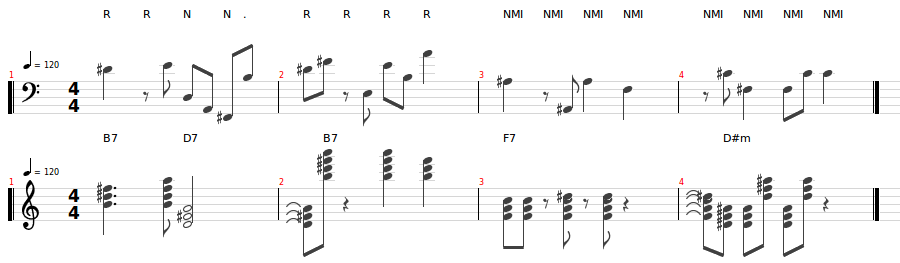
\includegraphics[width=\textwidth]{img/bassmatch.png}
\end{figure}
In questa figura possiamo notare come strumenti con un numero maggiore di pattern siano
più "musicali" e meno "casuali" all'orecchio di un ascoltatore.\\
Inoltre possiamo notare come le basi teoriche musicali
di coesione tra i vari musicisti siano state ben implementate.

\subsection{Algoritmo a selezione naturale (genetico / evoluzionistico)}

L'algoritmo evoluzionistico segue invece scelte legate all'esperienza,
facendo apprendere all'algoritmo
\footnote{Uno dei possibili sviluppi futuri, se non il più stimolante da un
punto di vista informatico/tecnico è la possibilità di salvare l'apprendimento
di un singolo musicista nel database, in modo da creare apprendimenti misti,
o un apprendimento decisamente più profondo di un determinato genere.}
una determinata canzone. \footnote{come indicato nella sezione \ref{sec:evol_alg}}
\\
Il problema della valutazione del singolo individuo (o run) è risultato da un
punto teorico decisamente complesso, da un punto di vista pratico/sperimentale
questa tesi è stata confermata, i parametri di controllo della mutazione e
i parametri base di valutazione della SOM
\footnote{Self organizing map, la funzione di valutazione,
senza avere input umani a runtime, usa meccanismi basati sulla norma 2
o distanza euclidea.}
sono risultati decisamente delicati, producendo risultati diversi ad una minima
variazione "dell'ago della bilancia".

\todo{qua ci va la canzone pura}
\todo{qua l'immagine di confronto con l'output dell'algoritmo genetico}

Notiamo ad esempio come il risultato in questo caso sia molto più coerente al
concetto di composizione musicale.
è importante specificare che questo concetto è abbastanza soggettivo,
decisamente legato alla provenienza geografica e alla storia di ogni persona
come musicista o semplice ascoltatore, si potrebbe dire che, in un certo senso,
l'output ricorda la composizione di partenza.

Dalle varie esecuzioni si può notare come la curva logaritmica dell'algoritmo
evolutivo sia limitata ad un punto\footnote{circa il 63\% per un'improvvisazione
di 12 misure}, questo è un comportamento voluto
per essere in modo esplicito distanti dal concetto di riproduzione fedele di una
determinata composizione, rendendo quindi il tutto solamente, in un certo modo,
simile alla composizione in input.

Concludendo, i risultati sono stati decisamente positivi, la piattaforma, una volta
sviluppate le parti mancanti e perfezionandola potrebbe essere decisamente utile
come strumento di studio per la branca della musica computazionale, oppure
essere usata come strumento didattico per l'improvvisazione.
